\documentclass[12pt,aspectratio=169]{beamer}
% Set theme
\usetheme{metropolis}
% Place package includes Here
\usepackage{graphicx}
\usepackage{appendixnumberbeamer}
\usepackage{booktabs}
\usepackage{fontspec}
\defaultfontfeatures{Path=/Library/TeX/Root/texmf-dist/fonts/opentype/public/fontawesome/}
\usepackage{fontawesome}
\usepackage{pythontex}
\usepackage{hyperref}
\usepackage{svg}
\setbeamertemplate{caption}{\raggedright\insertcaption\par}
% Title and author
\title{fiasco: a Python interface to the\\CHIANTI atomic database}
\subtitle{Heliophysics Community Python Working Group Meeting\\LASP---Boulder, CO USA}
\date{13 November 2018}
\author{Will Barnes}
\institute{Department of Physics and Astronomy, Rice University\\Houston, TX USA}
\titlegraphic{\hfill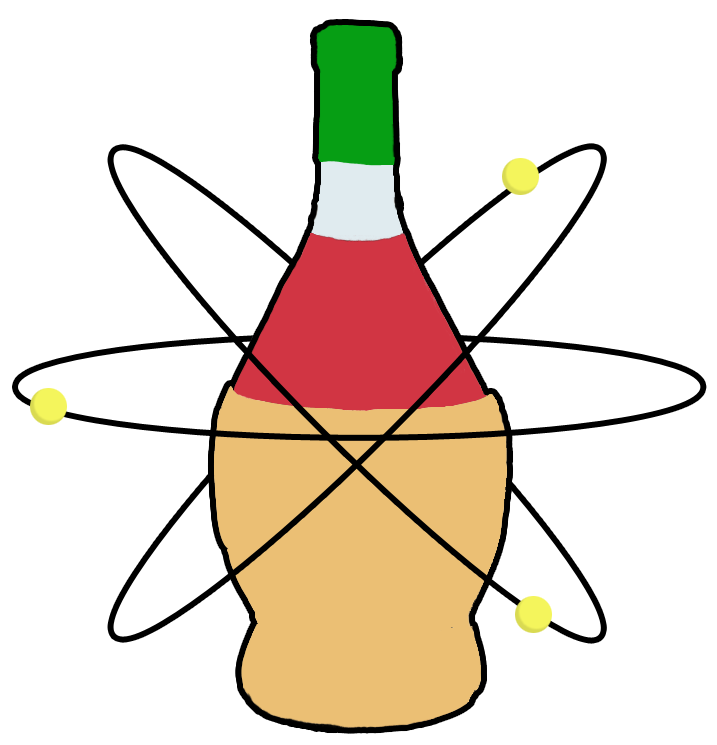
\includegraphics[height=1.5cm]{../figures/fiasco-logo.png}}

% Start Document
\begin{document}
% TeXFigure Manager
\begin{pycode}[manager]
import texfigure
manager = texfigure.Manager(pytex, '../figures')
\end{pycode}
% Title
\maketitle
% Contact
{%
\setbeamertemplate{frame footer}{\href{https://wtbarnes.github.io/heliopython-2018-talk}{wtbarnes.github.io/heliopython-2018-talk}}
\begin{frame}{Contact Info}
    \begin{itemize}
        \LARGE
        \item[]\faicon{github} \texttt{wtbarnes}
        \item[]\faicon{twitter} \texttt{wtbarnes\_}
        \item[]\faicon{envelope} \texttt{wtb2@rice.edu} 
        \item[]\faicon{globe} \texttt{wtbarnes.github.io}  
    \end{itemize}
\end{frame}
}
% Content
\begin{frame}
    \begin{figure}
        \centering
        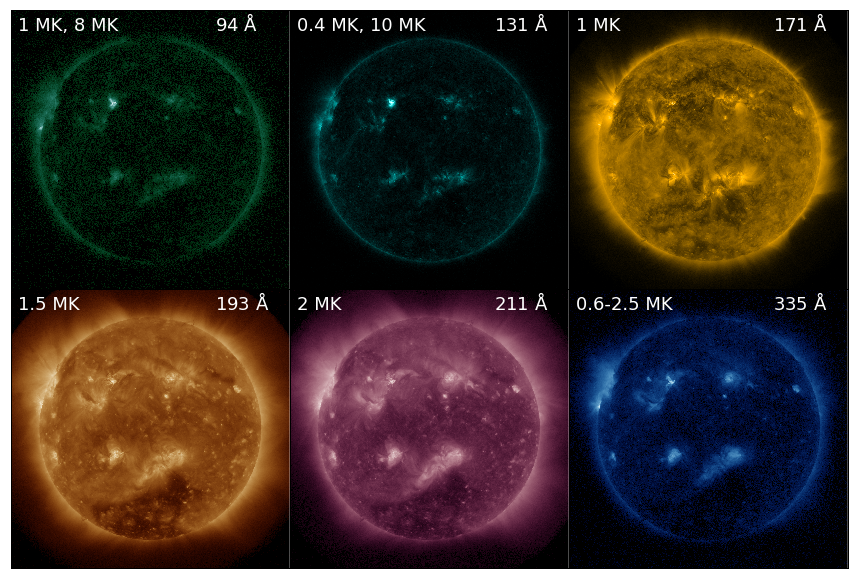
\includegraphics[width=0.9\textwidth]{../figures/aia_all_channels.png}
    \end{figure}
\end{frame}
%%
\section{The CHIANTI Atomic Database}
\begin{frame}[fragile]
    \begin{pycode}[manager]
import fiasco
import astropy.units as u
import roman
import pandas as pd
import plasmapy.atomic
import matplotlib.pyplot as plt
import matplotlib.colors
import seaborn
# Get all ions
ion_list = []
for el_name in fiasco.list_elements():
    el = fiasco.Element(el_name,[1e6]*u.K)
    for ion in el:
        if ion._elvlc is None:
            continue
        ion_list.append({'Element': el.atomic_symbol,
                         'Stage': roman.toRoman(ion.ionization_stage),
                         'Levels': ion[-1].level,})
# Create Table
ion_table = pd.DataFrame(ion_list)
ion_table_pivot = ion_table.pivot('Element','Stage','Levels')
new_indices = sorted(ion_table_pivot.index, key=lambda x:plasmapy.atomic.atomic_number(x))
ion_table_pivot = ion_table_pivot.reindex(new_indices)
ion_table_pivot = ion_table_pivot.reindex_axis(sorted(ion_table_pivot.columns.tolist(),
                                                      key=lambda x:roman.fromRoman(x)),axis=1)
# Create heatmap
fig = plt.figure(figsize=(15,8))
ax=fig.gca()
my_cmap = plt.get_cmap('Blues')
my_cmap.set_bad(color='w')
seaborn.heatmap(ion_table_pivot,
                ax=ax,
                square=False,
                cmap=my_cmap,
                annot=True,
                fmt='.0f',
                norm=matplotlib.colors.LogNorm(vmin=1,vmax=1e3),
                cbar_kws={'ticks':[1,10,100,1000]},
                cbar=False)
ax.tick_params(axis='both',which='both',bottom='off',left='off')
Fig_chianti_ptable = manager.save_figure('Fig_chianti_ptable', fext='.pdf')
    \end{pycode}
    \py[manager]|Fig_chianti_ptable|
\end{frame}
%%
\begin{frame}{The CHIANTI Database}
    \begin{itemize}
        \item Began around 1994, collaboration between multiple institutions (U. Cambridge, GMU, NRL, U. Michigan,...)
        \item Data and code distributed freely as tarball or via SSW
        \item Database: ~1.7 GB of plaintext (many thousands of files)
        \item Software
        \begin{itemize}
            \item Parses data; computes rates, population fractions, spectra, etc.
            \item Collection of useful IDL scripts
            \item Lacking: automated tests, documentation, version control, backwards compatibility
            \item \alert{No clear way to contribute code or report bugs!}
        \end{itemize}
        \item \textbf{ChiantiPy} first released in 2006 by K. Dere to provide Python interface to CHIANTI
    \end{itemize}
\end{frame}
%%
\begin{frame}[fragile]{The \emph{fiasco} Package}
\begin{columns}
    \column{0.7\textwidth}
        \begin{itemize}
            \item Scope largely same as IDL tools, ChiantiPy
            \item \alert{Python 3.6+ only}
            \item Licensed under BSD 3-Clause License
            \item Developed openly on \textbf{GitHub}
            \item Documentation builds on \textbf{Read the Docs}
            \item Automated test suite run on \textbf{Travis CI}
            \item Pre-v0.1--conda and pip packages coming soon(ish)
        \end{itemize}
        {\footnotesize
        \begin{pygments}{bash}
> git clone https://github.com/wtbarnes/fiasco.git
> cd fiasco && python setup.py install 
        \end{pygments}
        }
    \column{0.3\textwidth}
        \begin{figure}
            \centering
            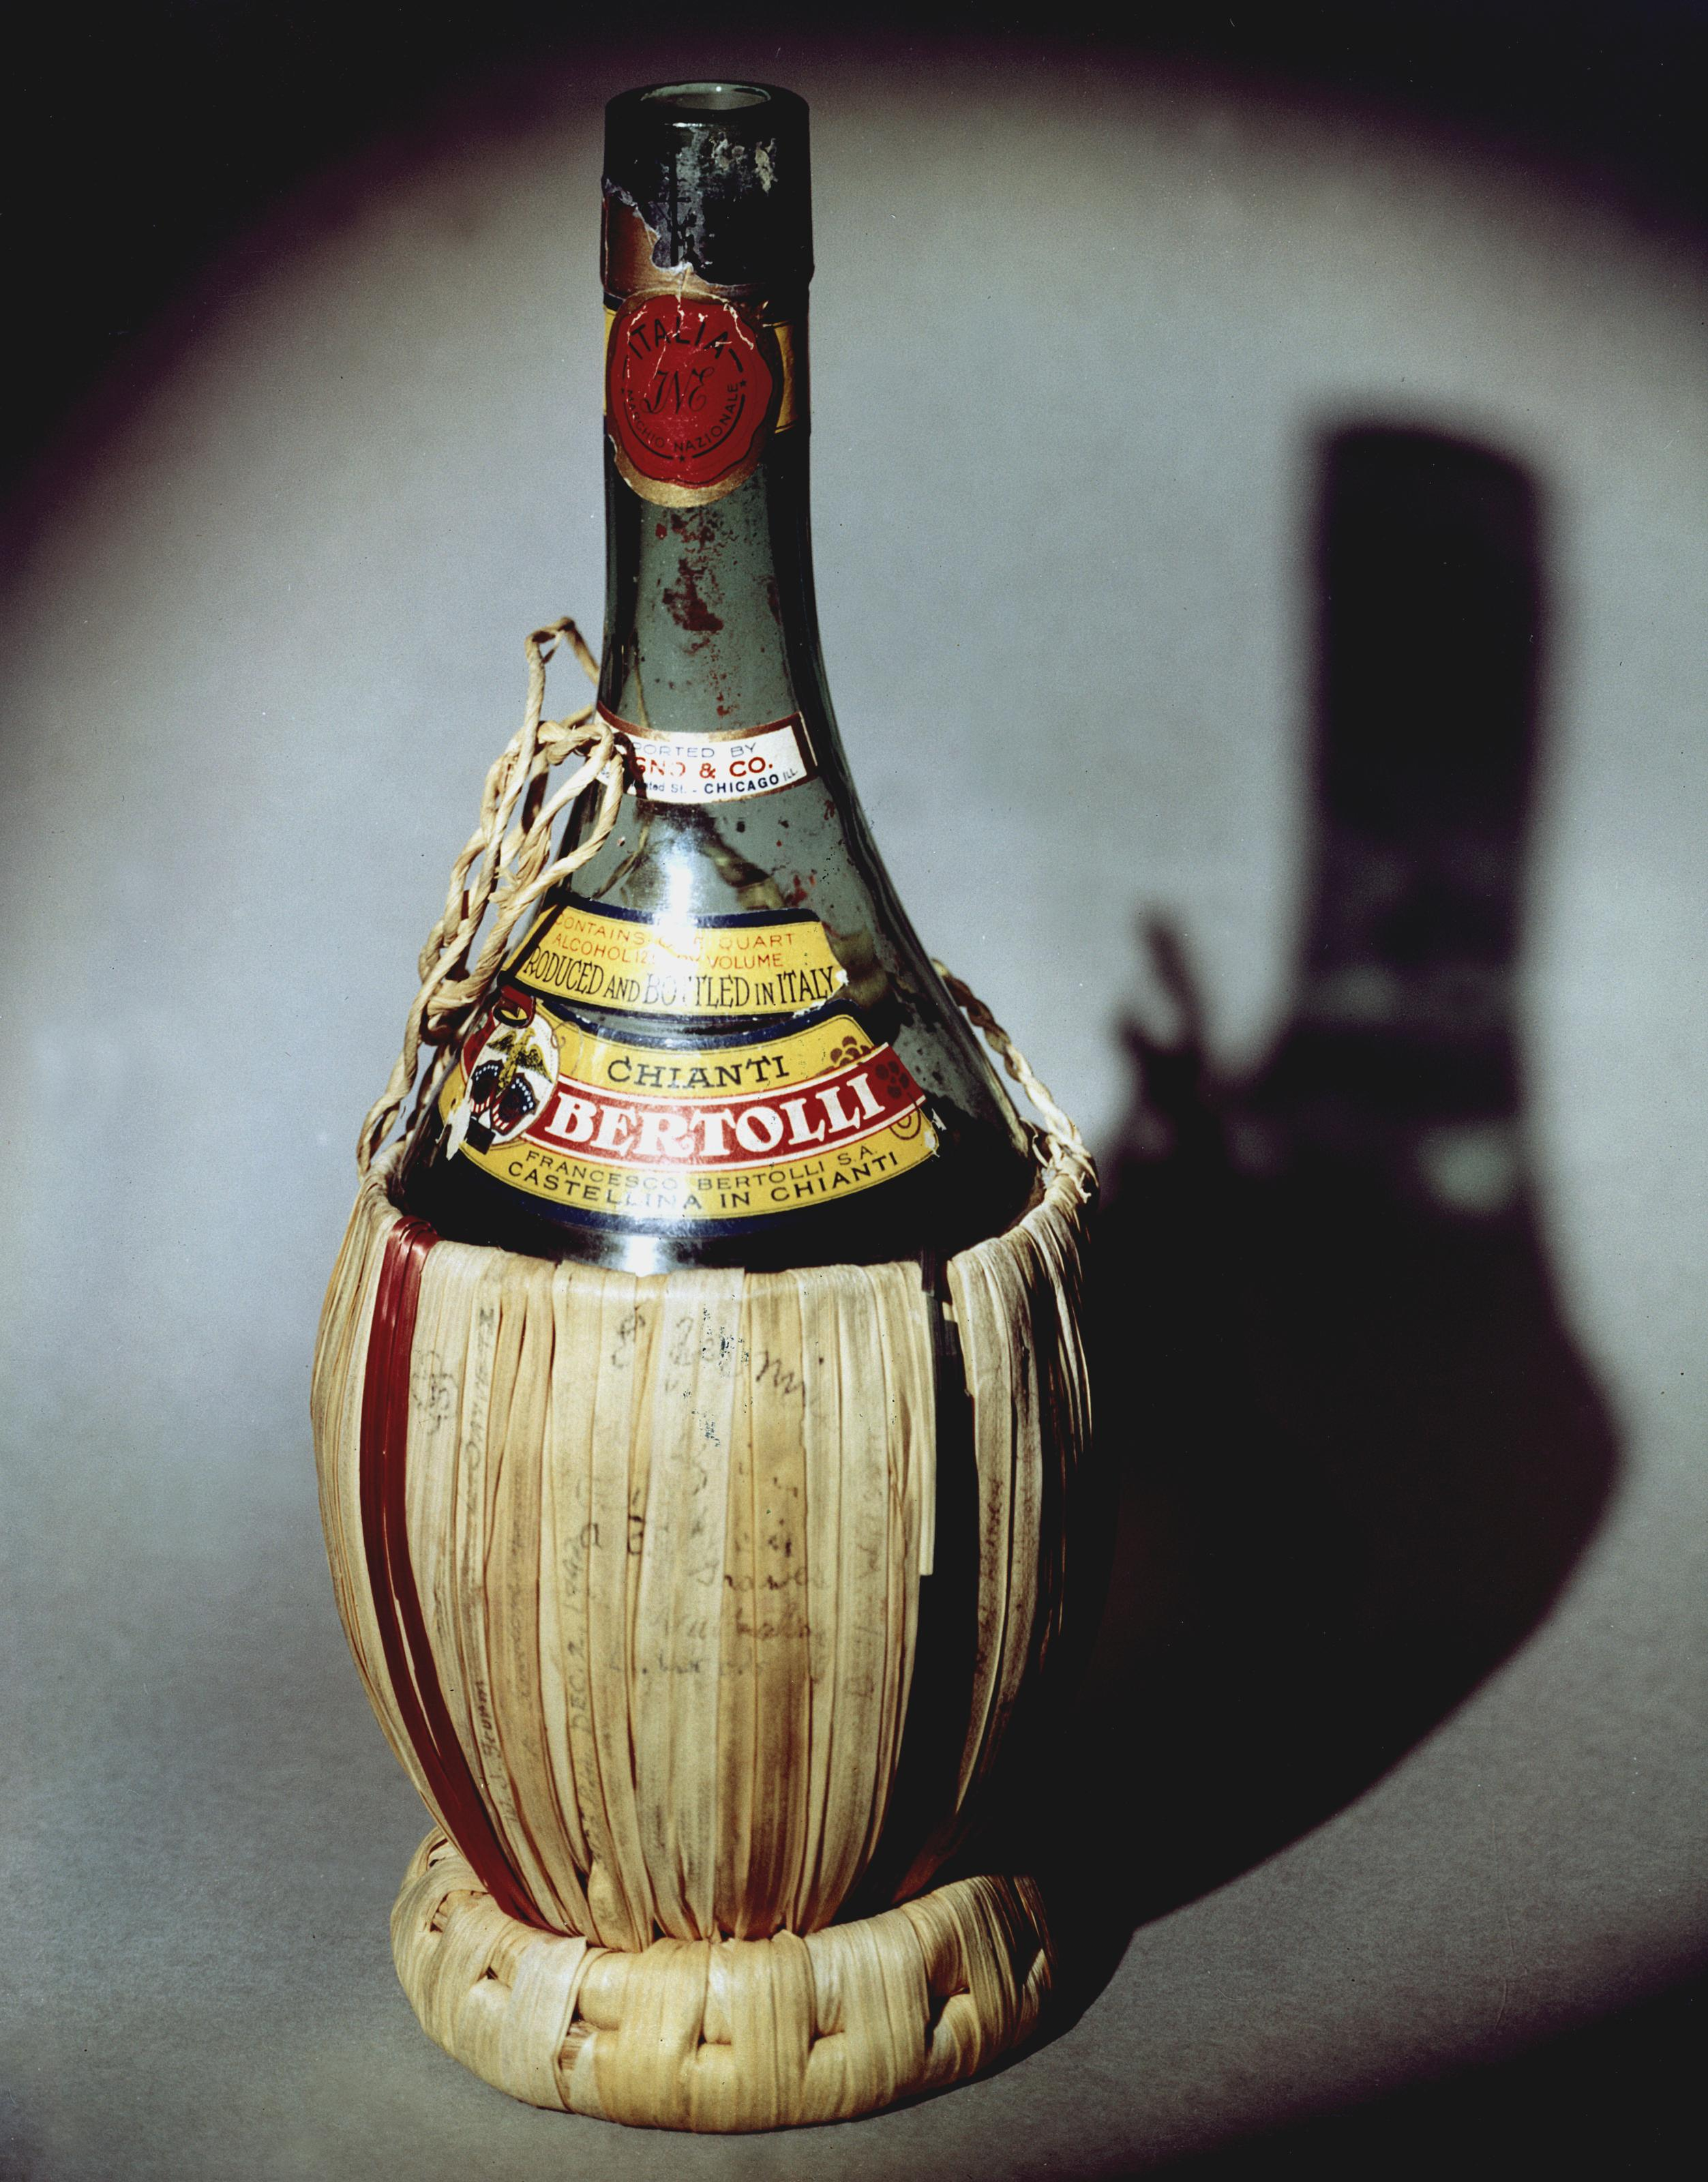
\includegraphics[width=\columnwidth]{../figures/chianti_bottle}
            \caption{}
        \end{figure}
\end{columns}
\end{frame}
%%%
\section{Parsing the Data}
%%
\begin{frame}[fragile]{Many Types of Files...}
    \scriptsize
    \begin{pygments}{bash}
        > tree ~/.fiasco/chianti_dbase/fe
            ├── fe_1
            │   └── fe_1.diparams
            ├── fe_10
            │   ├── fe_10.diparams
            │   ├── fe_10.drparams
            │   ├── fe_10.easplom
            │   ├── fe_10.easplups
            │   ├── fe_10.elvlc
            │   ├── fe_10.fblvl
            │   ├── fe_10.psplups
            │   ├── fe_10.rrparams
            │   ├── fe_10.scups
            │   ├── fe_10.wgfa
            │   └── fe_10_all.scups
            ...
    \end{pygments}    
\end{frame}
%%
\begin{frame}[fragile]{...in Many (Slightly) Different Formats}
    \tiny
    \begin{pygments}{console}
> head -n 5 ~/.fiasco/chianti_dbase/fe/fe_10/fe_10.elvlc
1     3s2 3p5                           2  P    1.5          0.000          0.000
2     3s2 3p5                           2  P    0.5      15683.100      15683.000
3     3s 3p6                            2  S    0.5     289236.000     289236.000
4     3s2 3p4 3d                        4  D    2.5     388713.500     387464.000
5     3s2 3p4 3d                        4  D    3.5     388708.000     387566.000
    \end{pygments}
    \begin{pygments}{console}
> head -n 6 ~/.fiasco/chianti_dbase/fe/fe_10/fe_10.scups
1      2   1.429e-01  -1.000e+00   1.940e-01   12    2   1.798e+01
0.000e+00   4.698e-02   1.097e-01   1.977e-01   3.302e-01   5.520e-01   7.114e-01   8.313e-01   9.249e-01   9.610e-01   9.801e-01   1.000e+00
6.022e+00   5.880e+00   5.690e+00   4.830e+00   3.790e+00   2.400e+00   1.530e+00   9.460e-01   5.190e-01   3.610e-01   2.790e-01   1.940e-01
1      3   2.636e+00   1.371e-01   2.080e-01   12    1   1.246e+00
0.000e+00   1.467e-01   2.949e-01   4.448e-01   5.971e-01   7.541e-01   8.300e-01   8.778e-01   9.149e-01   9.319e-01   9.435e-01   1.000e+00
1.024e+00   1.111e+00   1.198e+00   1.116e+00   9.116e-01   6.303e-01   4.751e-01   3.751e-01   3.030e-01   2.745e-01   2.572e-01   2.080e-01
    \end{pygments}
    \begin{pygments}{console}
> head -n 10 ~/.fiasco/chianti_dbase/fe/fe_10/fe_10.drparams
1
26   10  2.0320e+03  1.0180e+04  4.6380e+04  1.6980e+05  4.4990e+05  7.8800e+05  0.0000e+00  0.0000e+00  0.0000e+00
26   10  5.3350e-04  1.8270e-03  4.8510e-03  2.7100e-02  8.2260e-02  3.1470e-01  0.0000e+00  0.0000e+00  0.0000e+00
-1
file:  fe_10.drparams
parameters for dielectronic recombination rate coefficients
Determined from the coefficients listed at:
http://amdpp.phys.strath.ac.uk/tamoc/DATA/RR/
These calculations have been performed by a collaboration of researchers at:
Auburn University, Rollins College, and the University of Strathclyde.
    \end{pygments}
\end{frame}
%%
\begin{frame}{Parser Factory}
    \begin{columns}
        \column{0.6\textwidth}
            \begin{itemize}
                \item Many filetypes with many "quirks"
                \item \texttt{ParserFactory} metaclass creates parser classes "on the fly"
                \item Filetype determines parser class using a \emph{factory pattern}
                \item In most simple case, parser class just provides
                \begin{itemize}
                    \item[-] headings
                    \item[-] units
                    \item[-] types
                    \item[-] descriptions
                \end{itemize}
            \end{itemize}
        \column{0.4\textwidth}
            \includegraphics[width=0.9\columnwidth]{../figures/parser_inheritance_diagram.pdf}
    \end{columns}
\end{frame}
%%
\begin{frame}[fragile]{Parser Factory}
\footnotesize
\begin{pyconsole}
from fiasco.io import Parser
p = Parser('fe_16.elvlc')
p.parse()[:3]
type(p)
\end{pyconsole}
\end{frame}
\begin{frame}[fragile]{Parser Factory}
\scriptsize
\begin{pyconsole}
from fiasco.io import Parser
p = Parser('al_6.psplups')
p.parse()[:3]
type(p)
print(p.parse().meta['footer'])
\end{pyconsole}
\end{frame}
%%
\begin{frame}{HDF5 as a Database}
    \begin{itemize}
        \item Repeatedly parsing plaintext files is annoying
        \item \textbf{Instead, use HDF5!}
        \begin{itemize}
            \item[-] Hierarchical Data Format
            \item[-] Entire filetree in a single binary blob
            \item[-] Python interface via \texttt{h5py} package 
        \end{itemize}
        \item Easily slice and select parts of data that you need
        \item Easily store metadata alongside the data
    \end{itemize}
\end{frame}
\begin{frame}[fragile]{HDF5 as a Database}
    \footnotesize
    \begin{pyconsole}
import h5py; from fiasco.io import Parser
p = Parser('fe_16.elvlc'); table = p.parse()
with h5py.File('chianti.h5', 'w') as hf:
    p.to_hdf5(hf, table)

from fiasco import DataIndexer
d = DataIndexer('chianti.h5', 'fe/fe_16/elvlc')
d.footer
d.version
'E_obs' in d
d['E_obs'][:3]
    \end{pyconsole}
\end{frame}
%%%
\section{The \texttt{Ion} Class}
%%
\begin{frame}[fragile]{The \texttt{Ion} Class}
\end{frame}
%%%
\section{Dealing with Multiple Ions}
%%%
\section{Looking Forward}
%%
\begin{frame}{Remote Data Access}
    \begin{figure}
        \centering
        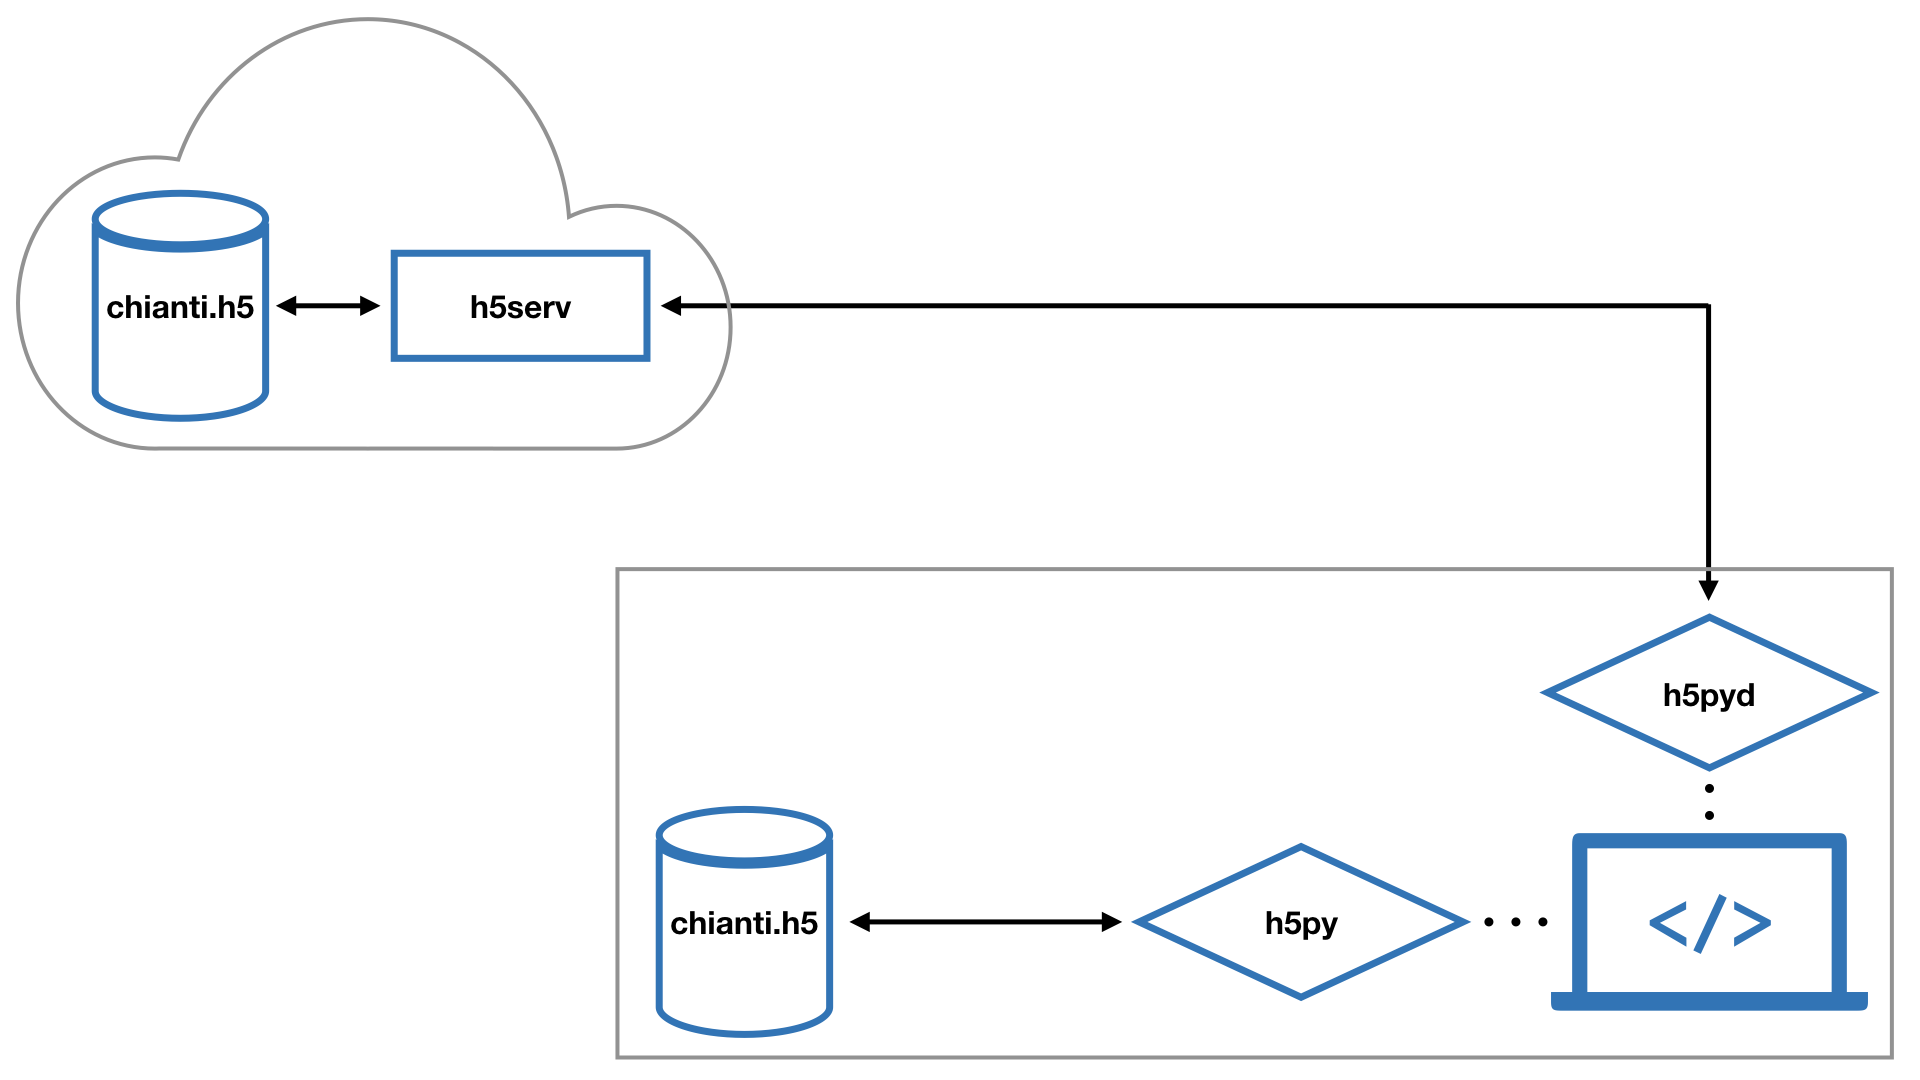
\includegraphics[width=0.95\textwidth]{../figures/cloud_diagram.png}
    \end{figure}
\end{frame}
%%%
{%
\setbeamertemplate{frame footer}{\href{https://wtbarnes.github.io/heliopython-2018-talk}{wtbarnes.github.io/heliopython-2018-talk}}
\begin{frame}{Resources}
    \begin{itemize}
        \LARGE
        \item[]\faicon{github} \texttt{wtbarnes/fiasco}
        \item[]\faicon{book} \texttt{fiasco.readthedocs.io}
        \item[]\faicon{globe} \texttt{chiantidatabase.org}   
    \end{itemize}
\end{frame}
}
%%
\begin{frame}{Acknowledgement}
    \begin{itemize}
        \item CHIANTI Team
        \item Ken Dere (ChiantiPy)
        \item SunPy Project (Stuart Mumford, David Pérez-Suárez)
        \item PlasmaPy Project (Nick Murphy, Drew Leonard)
        \item Stephen Bradshaw (Rice)
    \end{itemize}
\end{frame}
\end{document}
